\documentclass[aspectratio=169]{beamer}
\usepackage[utf8]{inputenc} 
\usepackage[T1]{fontenc}
\usepackage{lmodern}
\usepackage{amsmath, amssymb}
 \usepackage{caption}
 \usepackage{enumitem}
 \usepackage{caption}
\usepackage[french]{babel}
\usepackage{xcolor}
\usepackage{mathtools}
\setbeamersize{text margin left=0.1em} 
\setbeamersize{text margin right=0.1em} 
\usetheme{Boadilla}
\usecolortheme{seahorse}
\useoutertheme[left]{sidebar}
\setbeamertemplate{blocks}[rounded][shadow=true]
\title{Les reproducing kernel Hilbert spaces}
\subtitle{Présentation du TER, supervisé par Christophe Giraud}
\author[Matthieu Denis]{Matthieu Denis}
\date{\today}
\institute{Université Paris Saclay}
\begin{document}
	
\begin{frame}
	\titlepage
\end{frame}

\section{RKHS}

\begin{frame}
	\frametitle{Contexte}
	\begin{itemize}
		\item-\; $X$ un ensemble quelconque
		\item -\; $H$ un espace de Hilbert de fonctions réelles sur $X$
		\item -\; $\forall x \in X, \; L_x$ une forme linéaire sur $H$ : \[L_x : f \mapsto f(x) \; \forall f \in H\]
	\end{itemize}
\end{frame}

\begin{frame}
	\frametitle{Définitions}
		{\bf Définition : RKHS}\\
		
		 $L_x$ est bornée sur $H$, i.e :
		\[\forall x \in X, \;  \exists M_x > 0, \; \forall f \in H \text{ t.q } |L_x(f)| \coloneqq |f(x)| \leq M_x ||f||_H\]
\end{frame}

\begin{frame}
	\frametitle{Définitions}
	
	{\bf Définition : Noyau / Kernel}\\
	
	Une fonction $k : X \times X \to \mathbb{R}$ est un noyau si
	\[ \exists \phi : X \to H \text{ t.q } k(x,y) = \langle \phi (x), \phi(y) \rangle_H \; \forall x,y \in X \]
	
	\pause
	
	{\bf Définition : Noyau Reproduisant / Reproducing Kernel}\\
	
	Une fonction $k : X \times X \to \mathbb{R}$ est un noyau reproduisant de $H$ si $\forall x \in X, \, f \in H$ :
	\begin{itemize}
		\item[$\bullet$] $k(\cdot, x) \in H$			
		\item[$\bullet$] $f(x) = \langle f, k(\cdot, x) \rangle_H$
	\end{itemize}
\end{frame}

\begin{frame}
	\frametitle{Noyaux classiques}
	\begin{itemize}
		\item[$\bullet$] $k(x, y) \coloneqq \langle x, y \rangle$
		\item[$\bullet$] $k(x, y) \coloneqq (\alpha \langle x, y \rangle + 1)^d, \; \alpha \in \mathbb{R}, \; d \in \mathbb{N}$
		\item[$\bullet$] $k(x, y) \coloneqq \exp(||x-y||^2 / (2\sigma^2)), \; \sigma > 0$
		\item[$\bullet$] $k(x, y) \coloneqq \exp(||x-y|| / \sigma), \; \sigma > 0$
	\end{itemize}
\end{frame}

\begin{frame}
	\frametitle{Résultats importants}
	
	{\bf Propriété :}\\
	Noyau reproduisant $\Longrightarrow$ Noyau.
	
	\pause
	\bigskip
	
	{\bf Théorème :}\\
	$H$ est un RKHS $\Longleftrightarrow \exists !$ noyau reproduisant de $H$.
	
	\pause
	\bigskip
	
	{\bf Théorème de Moore-Aronszaj :}\\
	
	Soit $k$ un noyau. Alors $\exists !$ espace de Hilbert $H$ de fonctions sur $X$ pour lequel $k$ est un noyau reproduisant.
\end{frame}

\begin{frame}
	\frametitle{Application au ML : Le Representer Theorem}
	Soit $k$ un kernel sur $X$ et soit $H$ son RKHS associée. Posons $x_1, \cdots, x_n \in X$ notre training sample. Regardons le problème d'optimisation suivant :
	
	\[\min_{f \in H} \; J(f) \coloneqq E(f(x_1), \cdots, f(x_n)) + P(||f||_H^2)\]
	Où $P$ est une fonction croissante. \\
	
	Alors si ce problème d'optimisation a (au-moins) une solution, il y a (au-moins) une solution de la forme \[f = \sum_{i=1}^{n} \alpha_i \cdot k(\cdot, x_i)\]
	
	De plus, si $P$ est strictement croissante, alors toute solution a cette forme.
\end{frame}

\begin{frame}
	\frametitle{Kernel Ridge Regression}
	Ici, $J(f) \coloneqq \sum_{i=1}^{n} (y_i - f(x_i))^2 + \lambda ||f||_H^2$, prenons $k$ un kernel sur $X$. Le representer theorem nous dit que la solution de ce problème (sous couvert d'existence) est nécessairement de la forme 
	\[f = \sum_{i=1}^{n} \alpha_i \cdot k(\cdot, x_i)\]
	
	\pause
	
	\begin{align*}
		&\min_{f \in H} \; J(f) \coloneqq \sum_{i=1}^{n} (y_i - f(x_i))^2 + \lambda ||f||_H^2 \\
		\Longleftrightarrow& \min_{\alpha \in \mathbb{R}^n} \; \sum_{i=1}^{n} (y_i - \sum_{j=1}^{n} \alpha_j \cdot k(x_i, x_j))^2 + \lambda \sum_{i=1}^{n} \sum_{j=1}^{n} a_i a_j K(x_i, x_j) \\
		\Longleftrightarrow& \min_{\alpha \in \mathbb{R}^n} \; ||y - K \alpha||_2^2 + \lambda \alpha^T K \alpha \text{ avec $K_{ij} \coloneqq k(x_i, x_j)$}
	\end{align*}
\end{frame}

\begin{frame}
	\frametitle{SVM}
	Dans le cadre d'une SVM, $J(f) \coloneqq \frac{1}{n} \sum_{i=1}^{n} max(0, 1 - y_i f(x_i)) + \frac{\lambda}{2} ||f||_H^2$. Prenons un kernel $k$ sur $X$. Encore une fois, le representer theorem nous dit que la seule solution (si elle existe) est sous la forme
	\[f = \sum_{i=1}^{n} \alpha_i \cdot k(\cdot, x_i)\]
	
	\pause
	
	\[\min_{\alpha \in \mathbb{R}^n} \; \sum_{i=1}^{n} max(0, 1 - y_i \sum_{j=1}^{n} \alpha_j \cdot k(x_i, x_j))  + \frac{\lambda}{2} \sum_{i=1}^{n} \sum_{j=1}^{n} a_i a_j K(x_i, x_j) \]
	
	\pause
	
	On peut montrer que le dual de ce problème est :
	\[\min_{\gamma \in \mathbb{R}^n} \; -\sum_{i=1}^{n} \gamma_i + \frac{1}{2} \sum_{i=1}^{n} \sum_{j=1}^{n} \gamma_i \gamma_j y_i y_j k(x_i, x_j) \text{ t.q } 0 \leq \gamma_i \leq \frac{1}{n \lambda}, \; \alpha_i = y_i \gamma_i \forall i \]
\end{frame}

\begin{frame}
	\frametitle{Visualisation}
	\begin{center}
		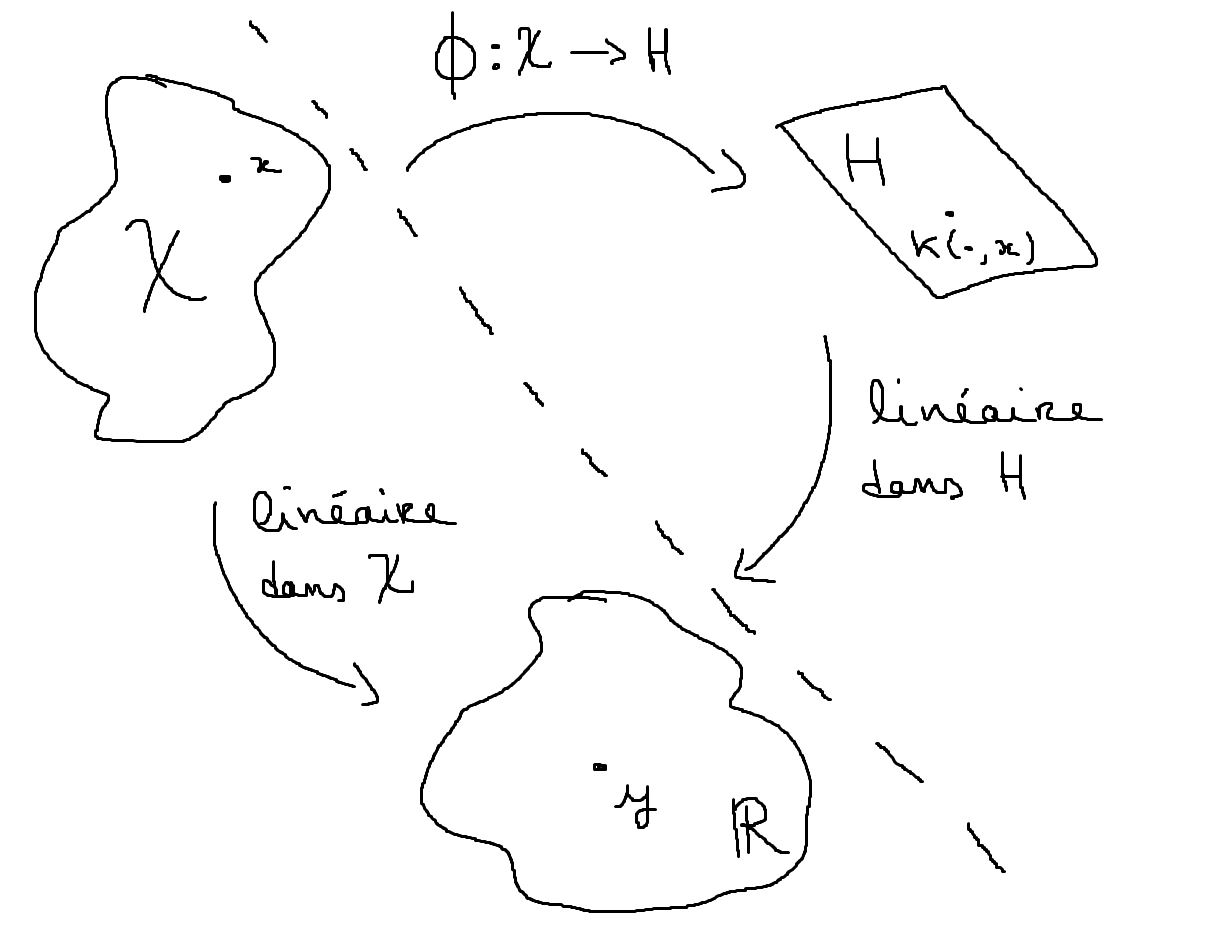
\includegraphics[width=9cm, height=6cm]{RKHS_schema.jpg} 
	\end{center}
\end{frame}

\begin{frame}
	\frametitle{Apparition des RKHS dans le cas d'un réseau de neurone simple}
	$\Phi : (\mathbb{R}^m \times \mathbb{R}^{m \times m} \times \mathbb{R}^m) \times \mathbb{R} \to \mathbb{R}$ combinaison d'applications linéaires, sans non linéarités  intermédiaires  :
	
	\[ \Phi ((\beta, A, u), x) \coloneqq \frac{1}{m^{\alpha}} \beta^T
	\left( \frac{1}{m^{\gamma}} A \right) u x \]
	
	\pause
	
	On initialise $\theta^0 \coloneqq (\beta^0, A^0, u^0)$ de manière standarde : 
	$ \forall i,j \in \{1, \cdots, m\} , \; u_i^0, A_{ij}^0, \beta_i^0 \sim_{iid} N(0, 1)$
\end{frame}

\begin{frame}
	\frametitle{Apparition des RKHS dans le cas d'un réseau de neurone simple}
	Posons une fonction de perte $F : \mathbb{R} \rightarrow \mathbb{R}$ t.q $F'(0) \neq 0$. Lorsque $\alpha < 1$, on a pour $m$ grand:
	
	\[||\nabla_{\beta / u / A} F(\Phi(\theta^{t+1}, x)) - \nabla_{\beta / u / A} F(\Phi(\theta^{t}, x)) || \ll ||\nabla_{\beta / u / A} F(\Phi(\theta^{t}, x))||\]
	
	\pause
	
	\[F(\Phi(\theta^{T}, x)) = F(\Phi(\theta^{0}, x)) + \langle \theta^{T}-\theta^0 , \nabla_{\theta} F(\Phi(\theta^0, x))  \rangle  + \mathcal{O}(m^{-1/2})\]
	
	\pause
	
	On apprend donc un modèle linéaire relatif aux features $\nabla_{\theta} F(\Phi(\theta^0, x))$, c'est-à-dire qu'après la transformation $x \rightarrow \nabla_{\theta} F(\Phi(\theta^0, x))$, on est linéaire. On fait donc face à un RKHS de noyau (par définition) 
	
	\[k(x,y)=\langle\nabla_{\theta} F(\Phi(\theta^0, x)),\nabla_{\theta} F(\Phi(\theta^0, y))\rangle \stackrel{LGN}{\longrightarrow} \mathbb{E}[\langle\nabla_{\theta} F(\Phi(\theta^0, x)),\nabla_{\theta} F(\Phi(\theta^0, y))\rangle]\]
\end{frame}


\end{document}